\documentclass[tikz,border=12pt]{standalone}
\usepackage[T1]{fontenc}
\usepackage{mathpazo}
\usepackage{amsmath,amssymb}
\usetikzlibrary{arrows.meta, positioning, calc, backgrounds}

\definecolor{stblue}{HTML}{7B97AD}
\definecolor{rwgold}{HTML}{B8995E}
\definecolor{sage}{HTML}{7A9A7E}
\definecolor{dkbrown}{HTML}{3D3530}
\definecolor{wmgray}{HTML}{7B7067}
\definecolor{cream}{HTML}{F9F6F0}
\definecolor{border}{HTML}{D4C9B8}
\definecolor{terracotta}{HTML}{C47A6A}
\definecolor{lavender}{HTML}{907EA0}
\definecolor{copper}{HTML}{A58B6D}

\begin{document}
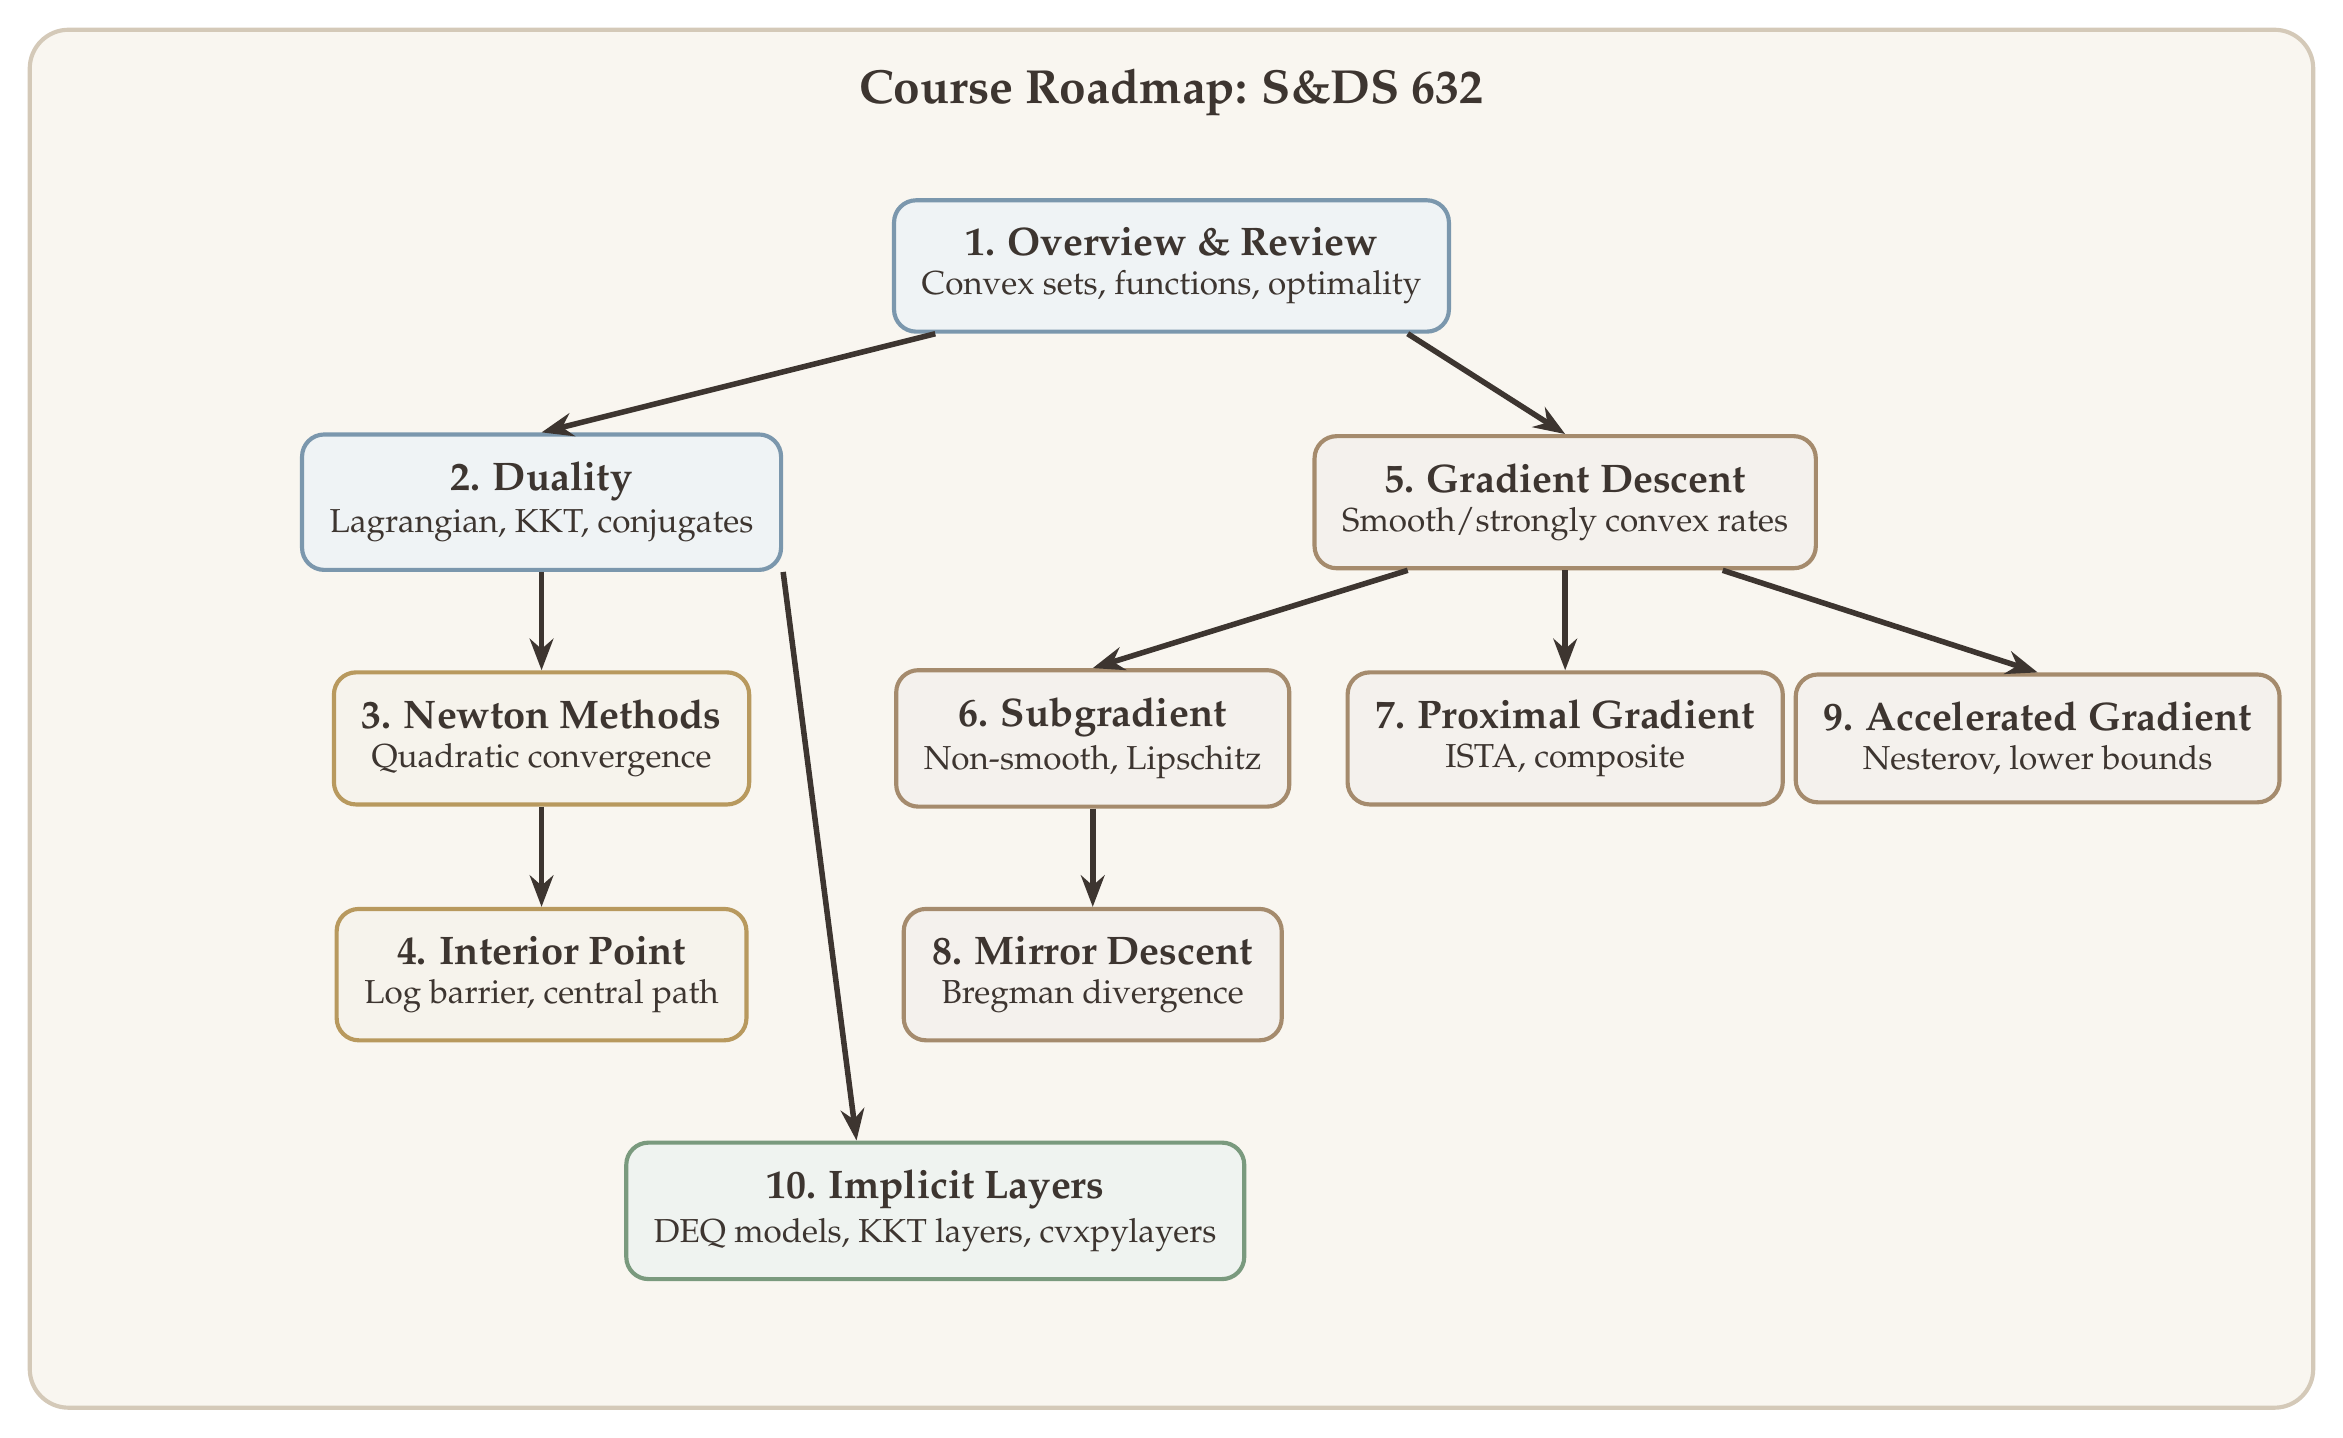
\begin{tikzpicture}[
  >={Stealth[length=4mm, width=3mm]},
  chbox/.style={rounded corners=8pt, line width=1.5pt, minimum height=1.6cm,
                minimum width=4.8cm, text=dkbrown, align=center, inner sep=10pt},
]

% Background
\fill[cream, rounded corners=14pt] (-1.5,-16) rectangle (27.5,1.5);
\draw[border, line width=1.5pt, rounded corners=14pt] (-1.5,-16) rectangle (27.5,1.5);

% Title
\node[font=\LARGE\bfseries, text=dkbrown] at (13,0.7) {Course Roadmap: S\&DS 632};

% === Row 0: Overview ===
\node[chbox, fill=stblue!12, draw=stblue, minimum width=7cm] (ch1) at (13,-1.5)
  {{\Large\bfseries 1. Overview \& Review}\\[2pt]{\large Convex sets, functions, optimality}};

% === Row 1: Two branches ===
\node[chbox, fill=stblue!12, draw=stblue] (ch2) at (5,-4.5)
  {{\Large\bfseries 2. Duality}\\[2pt]{\large Lagrangian, KKT, conjugates}};

\node[chbox, fill=copper!12, draw=copper] (ch5) at (18,-4.5)
  {{\Large\bfseries 5. Gradient Descent}\\[2pt]{\large Smooth/strongly convex rates}};

% Arrows from ch1 to ch2 and ch5
\draw[->, line width=2pt, dkbrown] ($(ch1.south)+(-3,0)$) -- (ch2.north);
\draw[->, line width=2pt, dkbrown] ($(ch1.south)+(3,0)$) -- (ch5.north);

% === Row 2: Newton + three first-order children of GD ===
\node[chbox, fill=rwgold!12, draw=rwgold] (ch3) at (5,-7.5)
  {{\Large\bfseries 3. Newton Methods}\\[2pt]{\large Quadratic convergence}};

\node[chbox, fill=copper!12, draw=copper] (ch6) at (12,-7.5)
  {{\Large\bfseries 6. Subgradient}\\[2pt]{\large Non-smooth, Lipschitz}};

\node[chbox, fill=copper!12, draw=copper] (ch7) at (18,-7.5)
  {{\Large\bfseries 7. Proximal Gradient}\\[2pt]{\large ISTA, composite}};

\node[chbox, fill=copper!12, draw=copper] (ch9) at (24,-7.5)
  {{\Large\bfseries 9. Accelerated Gradient}\\[2pt]{\large Nesterov, lower bounds}};

% Arrows from duality and GD to row 2
\draw[->, line width=2pt, dkbrown] (ch2.south) -- (ch3.north);
\draw[->, line width=2pt, dkbrown] ($(ch5.south)+(-2,0)$) -- (ch6.north);
\draw[->, line width=2pt, dkbrown] (ch5.south) -- (ch7.north);
\draw[->, line width=2pt, dkbrown] ($(ch5.south)+(2,0)$) -- (ch9.north);

% === Row 3: IPM + Mirror Descent ===
\node[chbox, fill=rwgold!12, draw=rwgold] (ch4) at (5,-10.5)
  {{\Large\bfseries 4. Interior Point}\\[2pt]{\large Log barrier, central path}};

\node[chbox, fill=copper!12, draw=copper] (ch8) at (12,-10.5)
  {{\Large\bfseries 8. Mirror Descent}\\[2pt]{\large Bregman divergence}};

\draw[->, line width=2pt, dkbrown] (ch3.south) -- (ch4.north);
\draw[->, line width=2pt, dkbrown] (ch6.south) -- (ch8.north);

% === Row 4: Implicit Layers ===
\node[chbox, fill=sage!12, draw=sage, minimum width=7cm] (ch10) at (10,-13.5)
  {{\Large\bfseries 10. Implicit Layers}\\[2pt]{\large DEQ models, KKT layers, cvxpylayers}};

\draw[->, line width=2pt, dkbrown] (ch2.south east) -- ($(ch10.north)+(-1,0)$);

% === Part region shading ===
\begin{pgfonlayer}{background}
  % Part I: Foundations
  \fill[stblue!5, rounded corners=10pt] (1.5,-0.5) rectangle (9,-5.5);
  \node[font=\large\bfseries, text=stblue!60] at (2.6,-0.8) {Part I};

  % Part II: Second-order
  \fill[rwgold!5, rounded corners=10pt] (1.8,-6.3) rectangle (8.2,-11.5);
  \node[font=\large\bfseries, text=rwgold!60] at (3,-6.6) {Part II};

  % Part III: First-order
  \fill[copper!5, rounded corners=10pt] (9.2,-3.3) rectangle (26.2,-11.5);
  \node[font=\large\bfseries, text=copper!60] at (10.4,-3.6) {Part III};

  % Part IV: Applications
  \fill[sage!5, rounded corners=10pt] (4.5,-12.3) rectangle (15.5,-14.7);
  \node[font=\large\bfseries, text=sage!60] at (5.8,-12.6) {Part IV};
\end{pgfonlayer}

\end{tikzpicture}
\end{document}
